\documentclass[dvipdfmx,autodetect-engine, unicode, 10pt, aspectratio=169]{beamer}

% \documentclass[dvipdfmx,autodetect-engine]{jsarticle}
% \usepackage{luatexja}% 日本語
% \usepackage[haranoaji,deluxe]{luatexja-preset}% フォント指定
\renewcommand{\kanjifamilydefault}{\gtdefault}% 既定をゴシック体に

\usetheme[progressbar=frametitle]{metropolis}
\usepackage{appendixnumberbeamer}
\usepackage{booktabs}
\usepackage[scale=2]{ccicons}
\usepackage{pgfplots}
\usepgfplotslibrary{dateplot}
\usepackage{xspace}
\newcommand{\themename}{\textbf{\textsc{metropolis}}\xspace}
\usepackage{adjustbox}
\usepackage{caption}
\captionsetup[figure]{font=tiny}
\usepackage{fancyvrb} % verbatim replacement that allows latex
\usepackage{listings} % Setting for Code block
\usepackage{bm} % for Bold font in Math \bm
\usepackage{ascmac} % for textbox

\title{時系列解析}
\subtitle{証券アナリスト}
% \date{\today}
\date{}
\author{Takayuki Suzuki}
\institute{This is institude of the author}

\begin{document}

\maketitle


\begin{frame}{時系列解析目標}
    \begin{enumerate}
        \item 時系列データの基本概念1:自己相関
        \item 時系列データの基本概念1:定常性
        \item トレンドモデル
        \item 誤差の評価
        \item 自己回帰モデル
        \item 単位根過程・ランダムウォーク
        \item 実践のフロー
        \item 見せかけの回帰と共和分
    \end{enumerate}
\end{frame}



\begin{frame}{自己相関}
    自己相関(Autocorrelation)は、系列相関(Serial Correlation)ともいう。\\
    相関でなく分散を指す場合、自己分散とか、自己共分散とかいう場合もある。\\
    基本的には同一の概念。\\
    時系列データ
    \begin{align*}
        Y_t =  \{ y_1, y_2, \dotsc , y_t \}
    \end{align*}
    があった時、たとえば、Yと、Yをk時刻だけずらした系列
    \begin{align*}
        Y_{t-k} =  \{ y_{1-k}, y_{2-k}, \dotsc , y_{t-k} \}
    \end{align*}
    を作り、$Y_t$と$Y_{t-k}$の相関$\text{Corr}(Y_t, Y_{t-k})$を考える。\\
    このように時刻をずらした自分自身との相関のことを、自己相関という。\\
    自己相関はラグkの関数であるが、どのようなときに自己相関が大きくなるか? 
\end{frame}

\begin{frame}{自己相関}
\footnotesize 
\begin{enumerate}
    \item トレンドがあり、増加を続ける、または減少を続ける場合。この場合ラグkの値に関わらず相関が大きくなる
    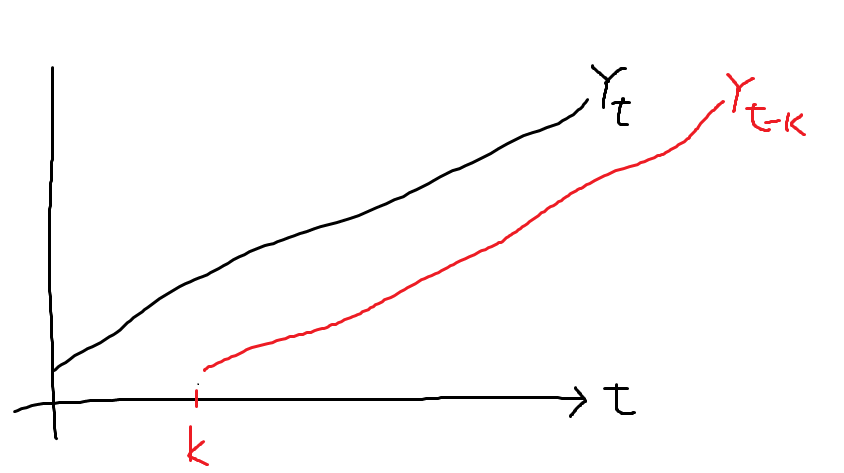
\includegraphics[width=0.4\linewidth]{trand.png}
    \item 周期性がある場合。この場合ラグkが周期と一致した場合に相関がおおきくなる
    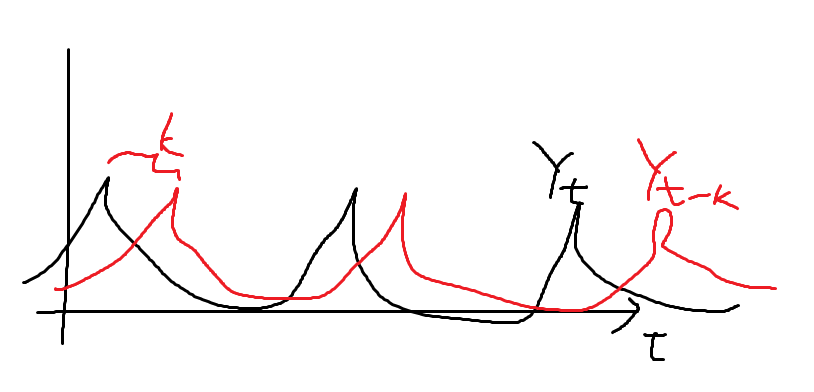
\includegraphics[width=0.4\linewidth]{periodic.png}
\end{enumerate}
\end{frame}

\begin{frame}{コレログラム}
    コレログラムとは、自己相関をラグKの関数とみて、横軸にラグk、縦軸に相関係数の図を書いたものである。
    前ページの例では、下記のようになる。
    \begin{enumerate}
        \item ラグkの値に関わらず相関は大きい\\
        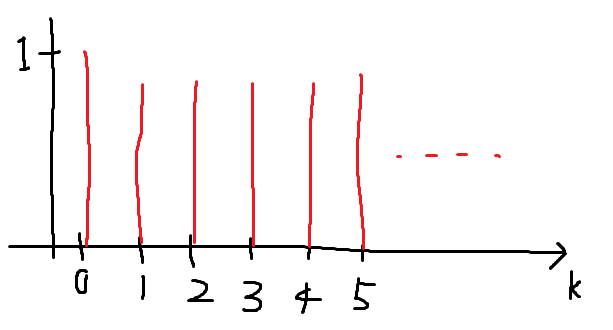
\includegraphics[width=0.3\linewidth]{correlogram_trend.png}
        \item ラグkが周期と一致した場合に相関が大きくなる(下記図は周期が3の場合)\\
        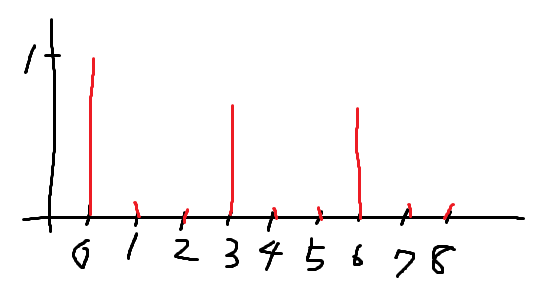
\includegraphics[width=0.3\linewidth]{correlogram_periodic.png}
    \end{enumerate}
    k=0の時は相関=1である点に注意。
\end{frame}

\begin{frame}{定常性}
    時系列データが下記3つの条件を満たすとき、そのデータは定常性を持つ、あるいは定常過程であるという。
    図はダメな例。
    \begin{itemize}
        \item 平均$\text{E}(y_t)$がすべてのtに対して等しい\footnotesize (トレンドが有る場合は平均がtによって変わるのでダメ)\\
            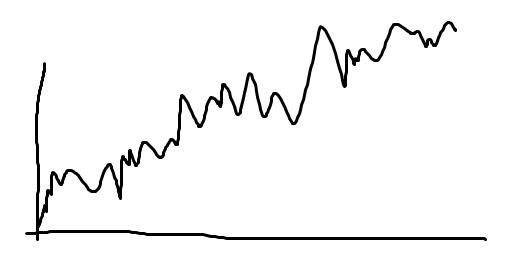
\includegraphics[width=0.2\linewidth]{change_average.PNG}
        \item 分散$\text{V}(y_t)$がすべてのtに対して等しい\footnotesize (ボラティリティが変わったらダメ)\\
            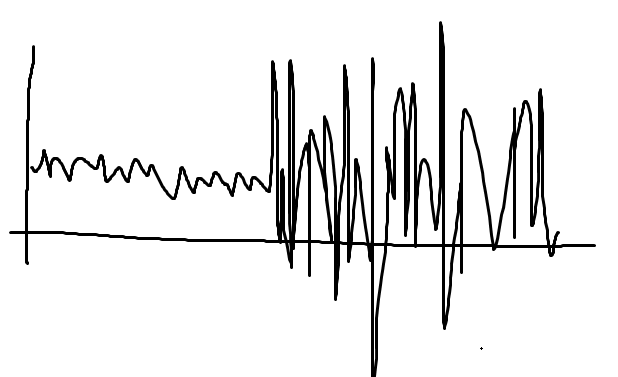
\includegraphics[width=0.2\linewidth]{varianve_change.PNG}
        \item 自己分散がラグkのみに依存し、時刻tに依存しない\footnotesize (周期性が変わったらダメ)\\
            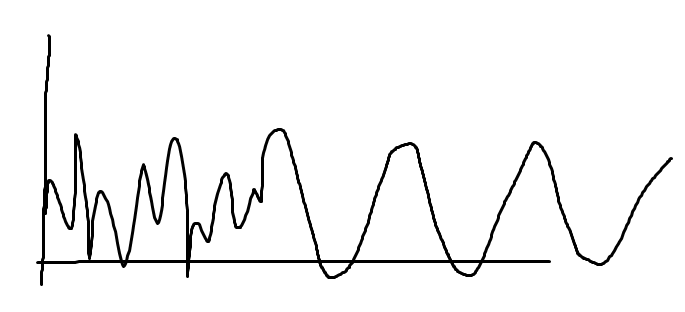
\includegraphics[width=0.2\linewidth]{change_periodic.PNG}
    \end{itemize}
    
\end{frame}

% \begin{frame}{トレンドモデル}
%     下記のような時系列データを考える。 \\
%     \begin{align*}
%         Y =  \{ y_1, y_2, \dotsc , y_t \}
%     \end{align*}
%     このデータを、モデルに当てはめて分析、予測を行う。 \\
% \end{frame}
\begin{frame}{トレンドモデル}
    トレンドモデルは、データの期待値が、時刻の一次関数で変化すると仮定したモデルである。
    数式にすると、下記のようなモデルである。 
    \begin{align*}
        y_t = \alpha + \beta t + \epsilon_t
    \end{align*}
    ここで、$t$は時刻、$\alpha, \beta$は回帰係数, $\epsilon$は誤差項である。\\
    トレンドモデルは、左辺を自然対数にした、対数トレンドモデルも採用されることがある
    \begin{align*}
        \ln(y_t) = \alpha + \beta t + \epsilon_t
    \end{align*}
    推定には、ふつう最小二乗回帰(OLS, \underline{O}rdinary \underline{L}east \underline{S}quares)で行う。\\
    OLSは二乗誤差を最小化していることだけ理解しておけばよい。\\
    \footnotesize 推定に利用する期間を「インサンプル」、推定に利用しない期間を、「アウトサンプル」という。\\
    アウトサンプルではモデルの当てはまりを評価するために利用されることが多いようだ。
    \begin{center}
        \adjustimage{max size={0.5\linewidth}{0.9\paperheight}}{timeseries1.drawio.png} \\
    \end{center}

\end{frame}
\begin{frame}{トレンドモデルでの予測計算}

    試験では、推定された予測式が与えられ、それに基づき次期の予測を行う問題が出題されそう。できるようにしておく。
    (協会テキスト4章の練習問題、問1および問2)
    \begin{itembox}[i]{例題1}
        あるデータYについて、期間$T=1,2,\dotsc , 100$を用いて、トレンドモデルに当てはめた結果、下記のような結果を得た
        \begin{align*}
            y_t = \alpha + \beta t + \epsilon_t \\
            \text{ただし  } \alpha = 1000, \beta = 20.0, 
        \end{align*}
        このとき、$T=101$および$T=200$の予測値を求めよ.
    \end{itembox}
    計算すると、T=101のとき、3020, T=200のとき、5000 になる。\\
    誤差項は予測には不要であることに注意。
    % \begin{align*}
    %     \hat{y}_t = \hat{b}_0 + \hat{b}_1 t \hspace{20pt} (t = 1, \dotsc,T)
    % \end{align*}
\end{frame}

\begin{frame}{トレンドモデルでの予測計算2}
    \begin{itembox}[i]{例題2}
        あるデータYについて、期間$T=1,2,\dotsc , 100$を用いて、対数トレンドモデルに当てはめた結果、下記のような結果を得た
        \begin{align*}
            \ln(y_t) = \alpha + \beta t + \epsilon_t \\
            \text{ただし  } \alpha = 5.0, \beta = 0.003, 
        \end{align*}
        このとき、$T=101$および$T=200$の予測値を求めよ.
    \end{itembox}
    計算すると、T=101のとき、3071, T=200のとき、59874になる. \\
    左辺が自然対数になっているので、計算は$\exp \{5.0 + 0.003 \times 101\}$などを計算すればよい。\\
    \vspace{10pt} 
    \footnotesize 例題1と比べると、T=101の時の予測値はほぼ同じだが、T=200の予測値は大きく異なる。つまり時間が進むと誤差は大きくなることがある。
\end{frame}

\begin{frame}{誤差の評価:Durbin-watson比}
    残差の評価には、よくDurbin-watson比という値が用いられる。{\footnotesize(式は覚えなくてよい)}
    \begin{align*}
        DW = \frac{\sum_{i=1}^{t}(e_i - e_{i-1})^2}{\sum_{i=1}^{t}e_i^2} \hspace{10pt} \text{\footnotesize ただし$e$は残差(誤差)}
    \end{align*}
    これは考え方としては、残差のラグ1の自己相関を推定している。\\
    Durbin-watson比(DW)の値は0から4までの値を取る。
    \begin{itemize}
        \item DWが2であった場合、残差は自己相関(系列相関)を持たない
        \item DWが0であった場合、残差は正の100\%自己相関を持つ
        \item DWが4であった場合、残差は負の100\%自己相関を持つ
    \end{itemize} 
    残差が正/負の自己相関をもう、とはどういう意味か?
\end{frame}
\begin{frame}{誤差の評価:Durbin-watson比}
    例えば、下記の図のような予測を行った場合、DWは2よりも0に近い値になる。\\
    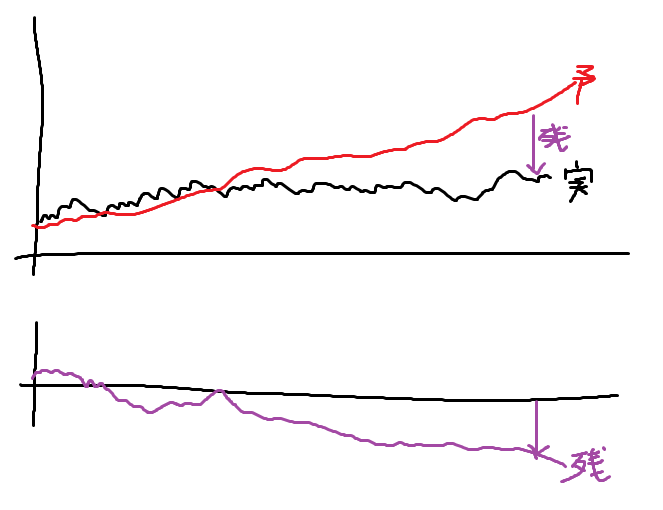
\includegraphics[width=0.5\linewidth]{DW4.png}\\
    なぜなら、残差が時間が増えると増加するトレンドがあり、つまり前の時刻の残差が大きいと次の時刻の残差も大きくなる傾向がある。
\end{frame}
\begin{frame}{誤差の評価:Durbin-watson比}
    つまり下記のように評価できる。
    \begin{itemize}
        \item DWが2より0に近い \\$\rightarrow$ 残差に正の系列相関があり、誤差が一度発生するとなかなか消えない傾向がある。
        \item DWが2より4に近い\\ $\rightarrow$ 残差に負の系列相関があり、残差に周期性がある事になる。
        \item DWが2に近い \\$\rightarrow$ 残差に系列相関はない。この場合のみ、残差は良い性質を持っていると言える。
    \end{itemize}
    \small トレンドモデルではしばしば、DWが4に近い値になり、残差が正の系列相関を持つ場合がある。なぜならトレンドモデルは一定の増加/減少トレンドがずっと続くと仮定しているモデルであるが、現実は様々な出来事がインパクトを与え、そのインパクトの影響は後々まで影響を与えるものであるから。だからDW比での誤差評価は、特にトレンドモデルの場合は重要である。

    \normalsize ⇒ ここまでの内容を用いて、協会テキスト例題4-1を解け
\end{frame}
\begin{frame}{自己回帰(AR)モデル}
    自己回帰(\underline{A}uto\underline{R}egression)モデル は、下記のようなモデルを仮定している。
    \begin{align*}
        y_t = \alpha + \beta y_{t-1} + \epsilon_t
    \end{align*}
    トレンドモデルとの違いは、第二項の変数が時刻tではなく、前期の自分の値$y_{t-1}$である点である。
    自己回帰モデルは前期だけでなく前前期、前前前期、。。。と好きなだけ変数を増やすことが原理上可能である。
    特に前記だけを用いたモデル(上記に書いたモデル)のことを、AR(1)モデルという。k期前までの値を利用したモデルは、AR(k)モデルという。
    
\end{frame}
\begin{frame}{ARモデルでの予想}
    AR(1)モデルの予測計算も出題されそう。
    \begin{itembox}[i]{例題3}
        あるデータYについて、期間$T=1,2,\dotsc , 100$を用いて、AR(1)モデルに当てはめた結果、下記のような結果を得た
        \begin{align*}
            y_t = \alpha + \beta y_{t-1} + \epsilon_t \\
            \text{ただし  } \alpha = 1000, \beta = 0.2, \\
            \text{また、$y_{100}=1200$であった。}
        \end{align*}
        このとき、$T=101$および$T=102$の予測値を求めよ.
    \end{itembox}
    計算すると、T=101のとき、$y_{101}=1240$, T=102のとき、$y_{102}=1248$になる。
\end{frame}

\begin{frame}{平均回帰水準}
    前記の予測を先の時刻まで続けてゆくと、だんだんある値に漸近してゆくことが分かる。\\
    この値のことを、平均回帰水準という。
    平均回帰水準は、ARモデルの$y$をすべて同一の$x$として一次方程式を解けば求まる。\\
    前ページの例の平均回帰水準は1250である。
    \begin{align*}
        x= 1000 + 0.2x \\
        \rightarrow x=1250
    \end{align*}
    ⇒ ここまでの内容で、協会テキスト例題4-2を解け。
\end{frame}
\begin{frame}{ランダムウォーク}
    実は全ページの計算では、平均回帰水準について言及していないことがあった。\\
    ARモデルの係数によっては、平均回帰水準が存在しないケースがある。実際、
    \begin{align*}
         y_t = \alpha + \beta y_{t-1} + \epsilon_t \\
         \text{ただし  } \alpha = 1000, \beta = 1.0,
    \end{align*}
    のような場合、平均回帰水準のための方程式(特性方程式)を立てると、
    $x = 1000 + x$となってしまい、解が一意に定まらない。このような場合を\bm{ランダムウォーク}といい、特に重要な意味を持つ。\\ \vspace{10pt}
    ランダムウォーク
    \begin{align*}
        y_{t}= \alpha + y_{t-1} + \epsilon
    \end{align*}
    なお定数項$\alpha$のことをドリフト項と呼ぶ。
\end{frame}
\begin{frame}{単位根検定}
    \small
    \begin{itemize}
        \item ある時系列データが、$\beta=1$の自己回帰モデルに従っている場合、その時系列データは「単位根を持つ」という。
        \item 単位根をもつなら平均回帰水準が存在せず、つまり平均値が時間によって変化する。つまり定常性を持たない
        \item 定常性を持たないデータはそのままトレンドモデルやARモデルを当てはめても、予測に利用することはできない。
    \end{itemize}
    \normalsize したがって、あるデータが単位根を持つか否かは、重要である。\\
    なお単位根を持つデータを分析するには、前期との差を取り「変化率」のデータにしてから分析すればよい。

\end{frame}
\begin{frame}{Dickey-Fuller検定}
    単位根を持つか否かは、基本的には$\beta=1$の帰無仮説を検定すればよいが、通常のt検定ではダメで、特別な検定方式を行う。その検定をDickey-Fuller検定という。\\
    特別ではあるが、t値やp値を閾値と比べて棄却する/有意とすることには変わらない。\\
    ⇒ 協会テキスト例題4-3を読め(解けなくてもよい)\\
    \vspace{10pt}
    ARCHモデルやGARCHモデルは出題されるとは思えないので割愛する。
\end{frame}
\begin{frame}{構造変化と季節性}
    ARモデルの実践としては、データを時系列プロットして、構造変化のある点を境にして、分析を分割する方法がある。\\
    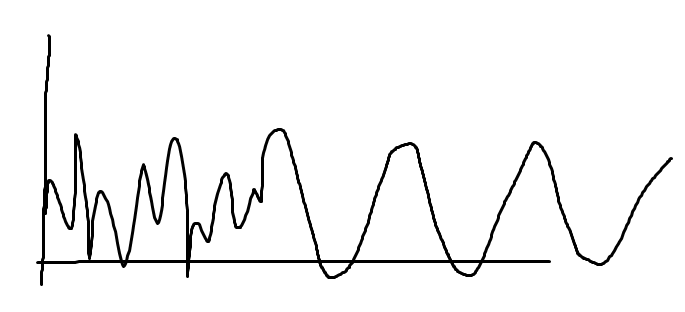
\includegraphics[width=0.4\linewidth]{change_periodic.PNG}\\
    他の実践として、データに季節性(つまり1年単位の周期性)が有る場合は、
    月次データの場合、ラグk=12の項を追加したARモデルで分析するケースがある。
    \begin{align*}
         y_t = \alpha + \beta_1 y_{t-1} + \beta_2 y_{t-12} + \epsilon_t \\
    \end{align*}
    こうすることで、年単位の周期性の因子をモデルに導入することができる。
\end{frame}
\begin{frame}{分析手順のフロー}
    \begin{figure}
        \centering
        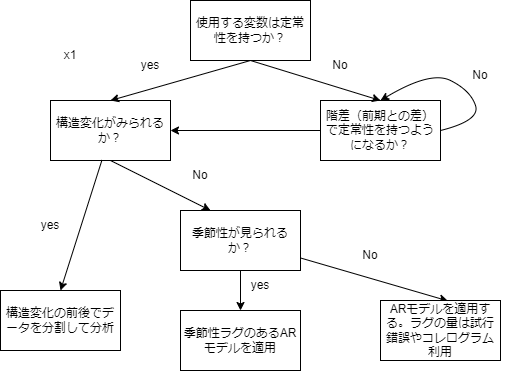
\includegraphics[width=0.65\linewidth]{correlogram.drawio.png}
        \caption{分析手順のフロー}
    \end{figure}
    
\end{frame}
\begin{frame}{見せかけの回帰と共和分}
    単位根過程の重要な性質として、見せかけの回帰がある。\\
    これは、まったく関係のない二つの単位根過程で回帰分析を行うと、まったく無関係にもかかわらず、回帰係数が統計的に有意にゼロでない回帰式が導かれてしまう、というもの。\\
    原理はともかく、
    \begin{itemize}
        \item 二つの単位根過程同士の回帰分析をすると、見せかけの回帰が起こるために普通は正しく分析ができない。
    \end{itemize}
    ということを覚えておくこと。これには例外があり、二つの単位根過程が「共和分関係」にある場合は見せかけの回帰が発生しない。
    共和分関係についてのこれ以上の内容はおそらく出題されないので割愛する。\\
    \vspace{10pt}
    ⇒ 協会テキスト 第4章の練習問題を解け。
\end{frame}

\end{document}
